\chapter{Evaluation} \label{chapter:Evaluation}
The following chapter first explains the setup behind the conducted tests. After that, the performance of the parallelized algorithms is measured and compared to their respective non-parallelized versions. The algorithms in test are Naive-Nested-Loops, Block-Nested-Loops, Divide-and-Conquer, ST-S and SARTS. 

\section{Setup}

%\subsection{Test Environment}
% pc specs
All the tests were conducted on a Lenovo E550 machine with the following technical specification: 
\begin{itemize}
	\item \textbf{CPU:} Dual core Intel Core i7-5500U with a 4096 KB cache
	\item \textbf{RAM:} 8 GB DDR3L 1600 MHz
	\item \textbf{Graphics:} Intel HD Graphics 5500
	\item \textbf{Operating System:} Linux Mint 18.2 Sonya 64-bit
\end{itemize}

% clean run
Before testing, the machine was newly rebooted in order to achieve a completely ``clean run'' for the tests. Any wired and wireless networking (WiFi, Bluetooth, etc.) has been switched off. Only the programs necessary for the tests have been started, including a Linux terminal and the C++ program running and measuring the algorithms. Any processes not related to the basic operating system maintenance with noticeable CPU or main memory usage have been killed. %The measured results were entered and stored on a different machine, so as to not influence the running measurements. Only algorithms required for the particular performance test were launched. 

% test setup (pipeline) explanation
Except for the Volcano version of BNL, all the algorithms were tested utilizing the produce/consume concept (section \ref{section:methods-frameworks}). A sample structure of the testing program is shown in Fig.~\ref{fig:test-setup}. 
At the beginning, the \textit{main} class of the program initializes the test with user input, which is the number of tuples $n$ and the number of dimensions $dim$. Then, also within \textit{main}, the objects required for the program to run, are instantiated. These include a random tuple \textit{generator}, the algorithms that need to be tested, as well as an \textit{output} object for each of the algorithms, which receives and prints the respective skyline. The \textit{output} object initializes an algorithm by calling \textit{produce()} on it and waiting for it to produce results. The algorithm, in its turn, receives its input by calling \textit{produce()} on the \textit{generator}. In order to simulate non-recurring database queries, the \textit{generator} creates $n$ random tuples with $dim$ different dimensions each, using a random number generator. The tuples are then ``pushed'' through the pipeline from the \textit{generator}, bypassing and being filtered by the particular algorithm, and reaching the\textit{ output} object in the end. The \textit{operator} interface implemented by every class in the program --- except for the main --- enables for an easy exchangeability of the algorithms. %This way, different tests can be conducted without major changes to the overall program structure. 

\begin{figure}[h]
\centering
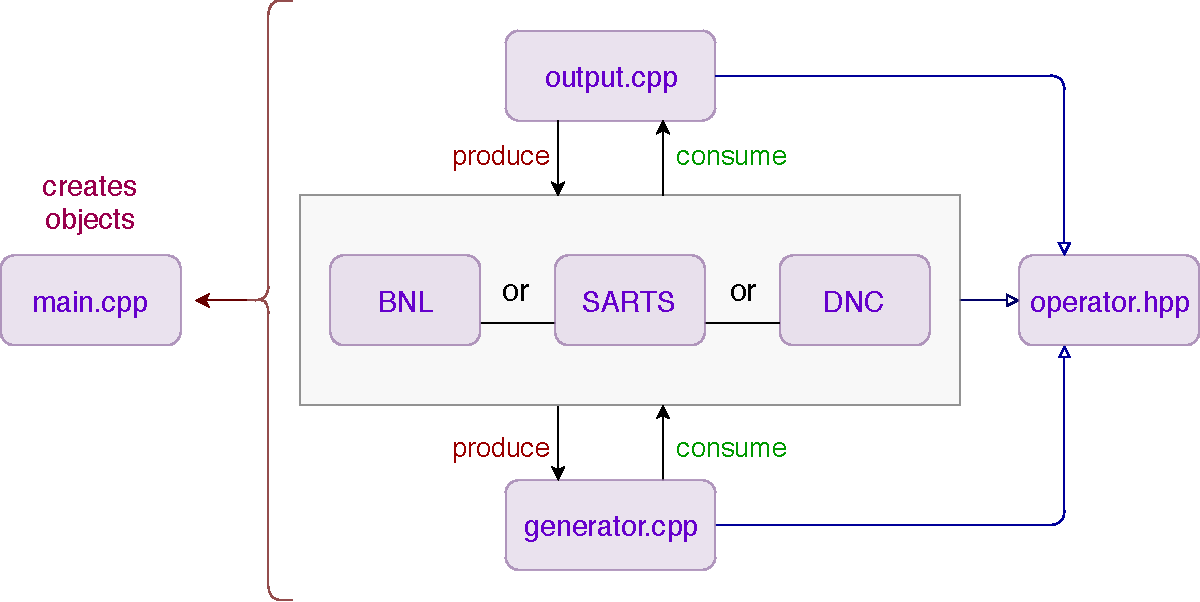
\includegraphics[width=0.9\linewidth]{figures/test-setup}
\caption{Test Setup with Sample Algorithms}
\label{fig:test-setup}
\end{figure}

While tree-based skyline algorithms, such as ST-S and SARTS, can only realistically work with categorical attributes, other general-purpose algorithms are not restricted to categorical attribute domains. Therefore, all tests that include the algorithms ST-S and SARTS were conducted using a limited set of integers as categories, ranging from 0 to 255. All other tests were performed with continuous attributes, represented as \textit{double} values. 

The memory usage of N-Tree and ART was captured with the tool Valgrind Massif. It is a heap profiler capable of determining how much heap memory the program is using at particular points in time. 

%\subsection{Measurement Metrics}
%The two metrics measured by performance tests were running time and main memory usage. For each of the running-time-entries within the test results, the median value from three independent test runs was taken, in order to reduce volatility of the results. 

%The two metrics measured by performance tests were running time and main memory usage. The running time was measured for all the algorithms in test, namely: BNL Volcano, BNL Produce/Consume, Naive Nested-Loops, parallel Naive Nested-Loops, DNC, parallel DNC, ST-S, parallel ST-S, SARTS and parallel SARTS. % adjust this list with respect to i/m and p/c
%The running time was captured in dependence of the number of tuples, the dimensionality of the input, as well as the number of threads that can be used in parallel. For each of the running-time-entries within the test results, the median value from three independent test runs was taken, in order to reduce volatility/variation of the results. 
%
%The main memory usage was measured for the N-Tree as well as for the ART tree, each in the scope of their respective algorithm ST-S or SARTS. 
%These measurements were conducted in dependence of the number of tuples and the dimensionality of the input. 
%
%While tree-based skyline algorithms, such as ST-S and SARTS, can only realistically work with categorical attributes, other general-purpose algorithms are not restricted to categorical attribute domains. Therefore, all tests that include the algorithms ST-S and SARTS were conducted using a limited set of integers as categories, ranging from 0 to 255. Other tests that do not include tree-based algorithms were performed with continuous attributes, represented as \textit{double} values in C++. 

%\subsection{Tools}
% Terminal Output
%When measuring the time taken to compute the skyline by each of the algorithms, the time point before the start of the algorithm and the time point after its finish were captured. The difference between the two points in time was interpreted as the running time of the particular algorithm. Any operations belonging to the environment of the algorithms, such as printing the output, generating the dataset, or freeing the memory after computation were \textit{not} included in their running time.  

% Valgrind Memcheck
%Before measuring the memory usage within ST-S and SARTS, it was made sure that no memory leaks exist in any of the two algorithms. This was done with the help of Valgrind Memcheck, which is a tool for memory error detection. 

% Valgrind Massif
%The main memory usage itself was captured with the tool Valgrind Massif. It is a heap profiler capable of determining how much heap memory the program is using at particular points in time. 
%This is done by making multiple snapshots of the heap's current state during runtime. In addition to that, at some points of program execution, which Massif considers especially relevant, it captures detailed snapshots, telling precisely which part of the code is responsible for which block of the allocated memory. 

\section{Results}
% expectations
%It is expected for the parallelized algorithms to outperform their sequential counterparts with a rising number of tuples and threads. In addition to that, the ART tree is supposed to show similar performance to the N-Tree in terms of running time, while having the advantage of lower space consumption. The two query pipelining models Volcano and produce/consume are expected to show mostly similar evaluation times. 
In the following, the results of the conducted measurements are presented. 

\subsection{Computation Time}
% Notes: 
% Bei jedem parallelisierten Algorithmus gibt es auch unparallelisierte Blöcke, die ganz normal skalieren. D.h. auch, dass die Performance nicht immer z.b. 4 x so gut ist wie nicht parallelisiert. z.b mutex, transport der tupel durch die pipeline, etc. 

\subsubsection{Volcano and Produce/Consume} \label{section:models-test-comparison}
To begin with, the two query pipelining approaches Volcano and produce/consume were compared to each other. For this purpose, two different variants of the Block-Nested-Loops algorithm were implemented. Both versions can be found in the Appendix \ref{appendix-code} to this work. 
% Bnl Volcano vs. Bnl produce/consume
\begin{figure}[h]
	\centering
	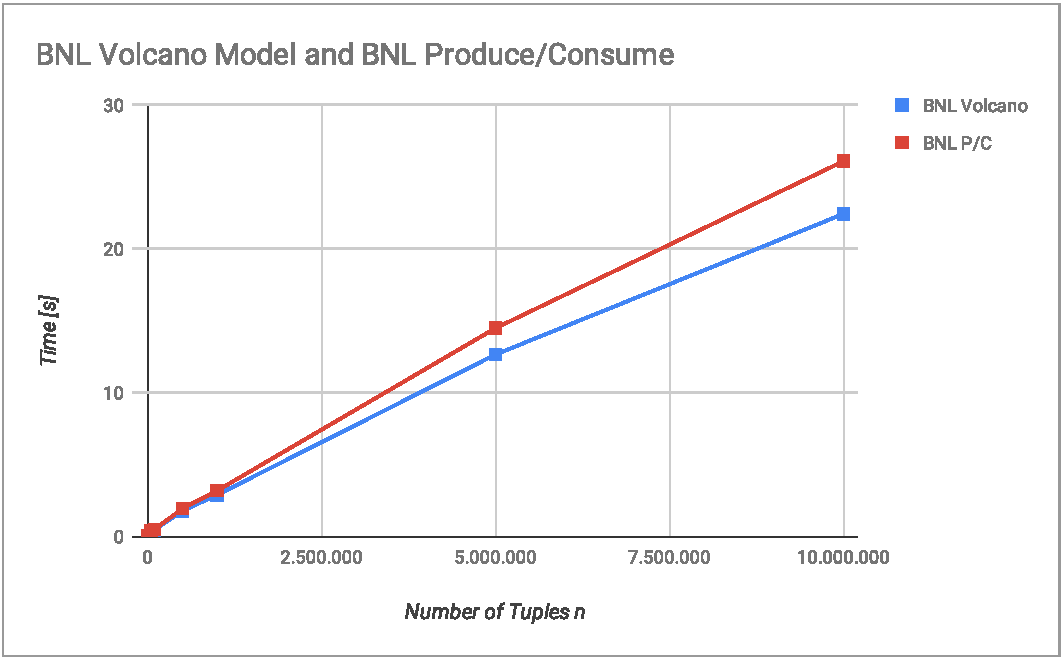
\includegraphics[width=1\linewidth]{figures/im-vs-pc}
	\caption{Comparison of Volcano Model and Produce/Consume Concept by Running Time}
	\label{fig:im-vs-pc}
\end{figure}
The results of the comparison (Fig.~\ref{fig:im-vs-pc}) show that up to a threshold of about 1 million tuples the running time of both BNL Volcano and BNL p/c is virtually the same. With the number of tuples further rising, the Volcano version consistently outperforms the produce/consume version. Therefore, the conclusion can be drawn that while the performance of Volcano is only slightly better than that of produce/consume, Volcano model is still the way to go for query pipelining. However, one should keep in mind that the produce/consume concept used in this work is not the original one, which would also include code generation, as explained in section \ref{section:methods-frameworks}. 
The underlying numbers to this comparison are given in form of a table in Appendix \ref{appendix-performance}. 

\subsubsection{Non-Progressive Algorithms}
Non-progressive skyline algorithms included in this work are Block-Nested-Loops and Divide-and-Conquer. In all three of the conducted tests, BNL proves that it scales significantly better than DNC. It shows overall better performance with rising numbers of tuples (Fig.~\ref{fig:non-progressive-n}), dimensions (Fig.~\ref{fig:non-progressive-dim}), and also threads (Fig.~\ref{fig:non-progressive-threads}). The same applies to the parallelized version of DNC. While it does perform better than the sequential version of DNC, it still cannot keep up with BNL in any of the tests. 

Herewith, the results are similar to the ones produced in the original paper \cite{kossmann}, where BNL and DNC were first introduced. In their evaluation, the authors showed that basic BNL significantly outperforms basic DNC for larger $n$. It is remarkable that the results measured within this work are significantly better than the results in \cite{kossmann} for both BNL and DNC. This is, however, not surprising, regarding the lack of I/O operations as well as a much more powerful testing machine this time. 

On the large scale of comparison between BNL and DNC, the two versions of BNL, namely Volcano style and Produce/Consume perform virtually the same in all three tests. There is, however, a slight difference between the two versions, as previously shown in this section. The concrete numbers measured within the tests can be found in Appendix \ref{appendix-performance}. 

% Non-Progressive Algorithms by n
\begin{figure}[h]
	\centering
	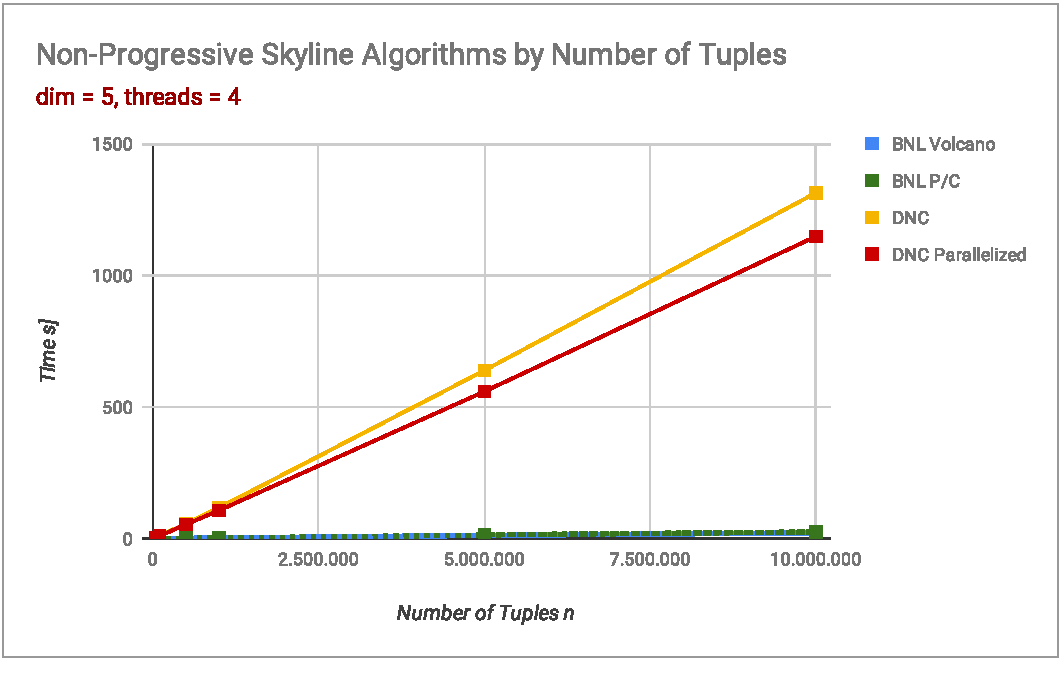
\includegraphics[width=1\linewidth]{figures/non-progressive-n}
	\caption{Running Time of Non-Progressive Algorithms by Number of Tuples}
	\label{fig:non-progressive-n}
\end{figure}

% Non-Progressive Algorithms by dim
\begin{figure}[H]
	\centering
	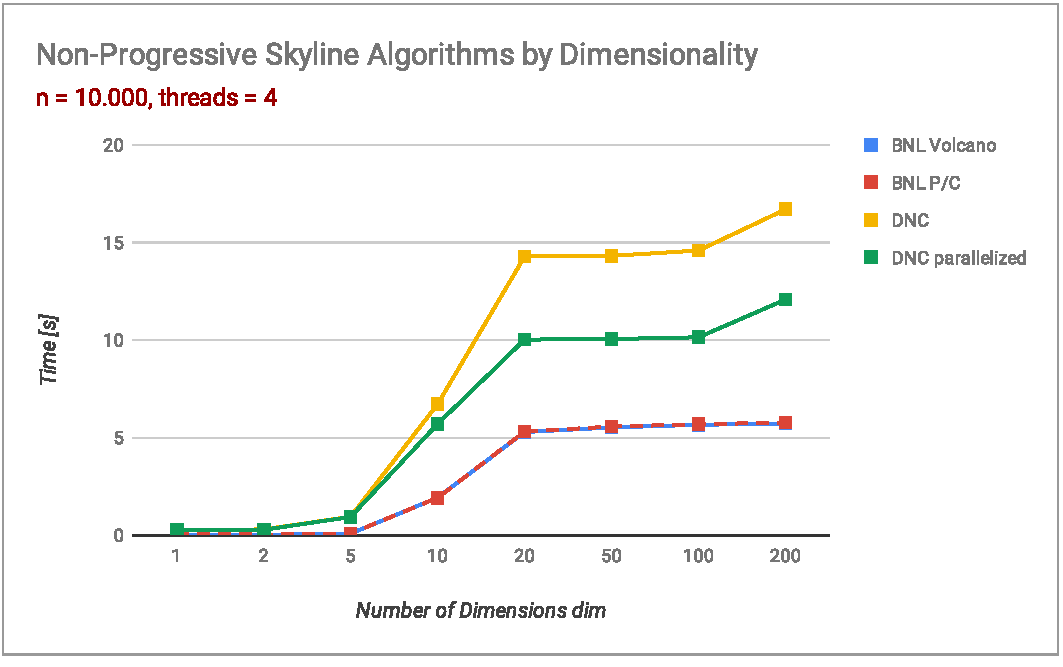
\includegraphics[width=1\linewidth]{figures/non-progressive-dim}
	\caption{Running Time of Non-Progressive Algorithms by Dimensionality}
	\label{fig:non-progressive-dim}
\end{figure}

% Non-Progressive Algorithms by threads
\begin{figure}[h]
	\centering
	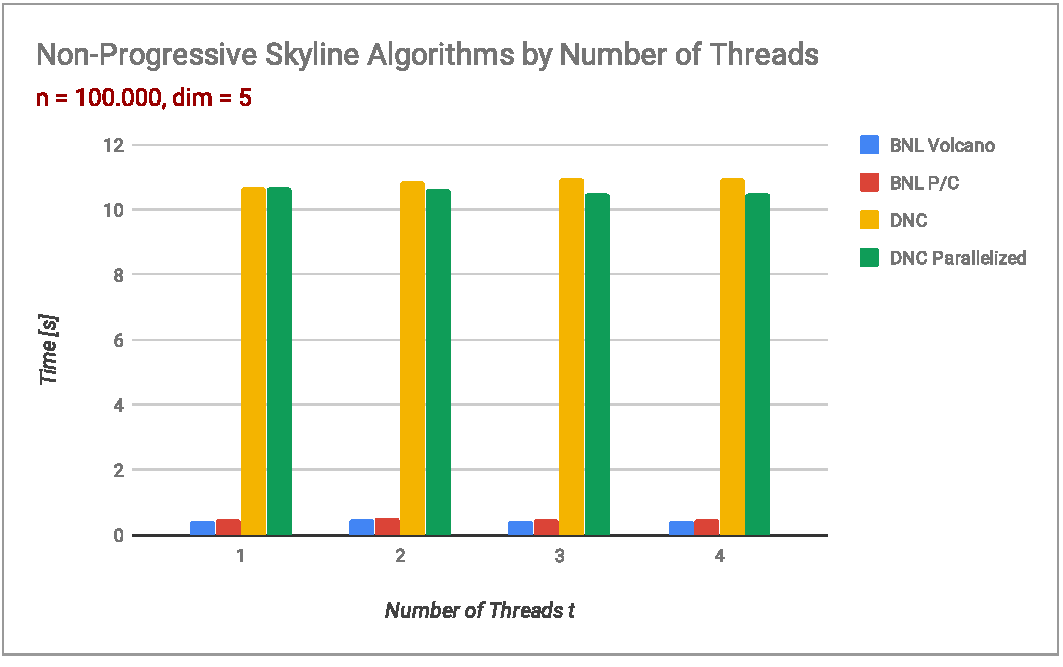
\includegraphics[width=1\linewidth]{figures/non-progressive-threads}
	\caption{Running Time of Non-Progressive Algorithms by Number of Threads}
	\label{fig:non-progressive-threads}
\end{figure}

\subsubsection{Progressive Algorithms}
Despite being the arguably simplest skyline algorithm to date, Naive-Nested-Loops can be both progressive and parallelizable if implemented correctly. This is what this work makes use of in order to make it comparable with the two newer algorithms ST-S and SARTS. 

As expected, for a rising number of tuples $n$ both ST-S and SARTS perform extremely well. As shown in Fig.~\ref{fig:progressive-n}, they significantly outperform Naive-Nested-Loops for both middle-range and large $n$. This is not surprising, considering that ST-S and SARTS were both specifically developed for large categorical datasets. It is due to the efficient tree structures used,  that dominance checks can be conducted very efficiently, and depend less on the number of tuples than on the dimensionality of the dataset (section \ref{section:art-characteristics}). 

% Progressive Algorithms by n
\begin{figure}[h]
	\centering
	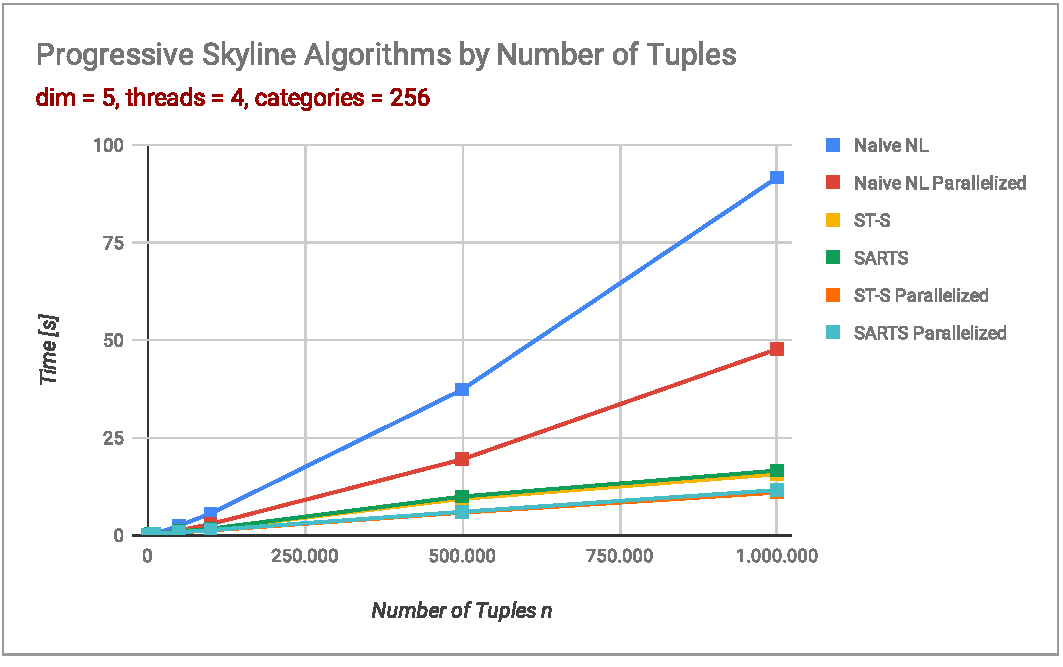
\includegraphics[width=1\linewidth]{figures/progressive-n}
	\caption{Running Time of Progressive Algorithms by Number of Tuples}
	\label{fig:progressive-n}
\end{figure}

A more close-up comparison of ST-S and SARTS is shown in Fig.~\ref{fig:progressive-n-2}. It can be seen that the parallelized versions of both algorithms start outperforming their sequential counterparts at a dataset size of about 100,000 tuples. While the ST-S and SARTS algorithms generally go ``hand-in-hand'' for both sequential and parallelized versions, the ST-S algorithm is slightly better than SARTS for large $n$. This advantage, however, seems of lesser significance in comparison to the memory usage gains of the SARTS algorithm, which will be presented in the next section of this work. 

% Progressive Algorithms by n - second
\begin{figure}[H]
	\centering
	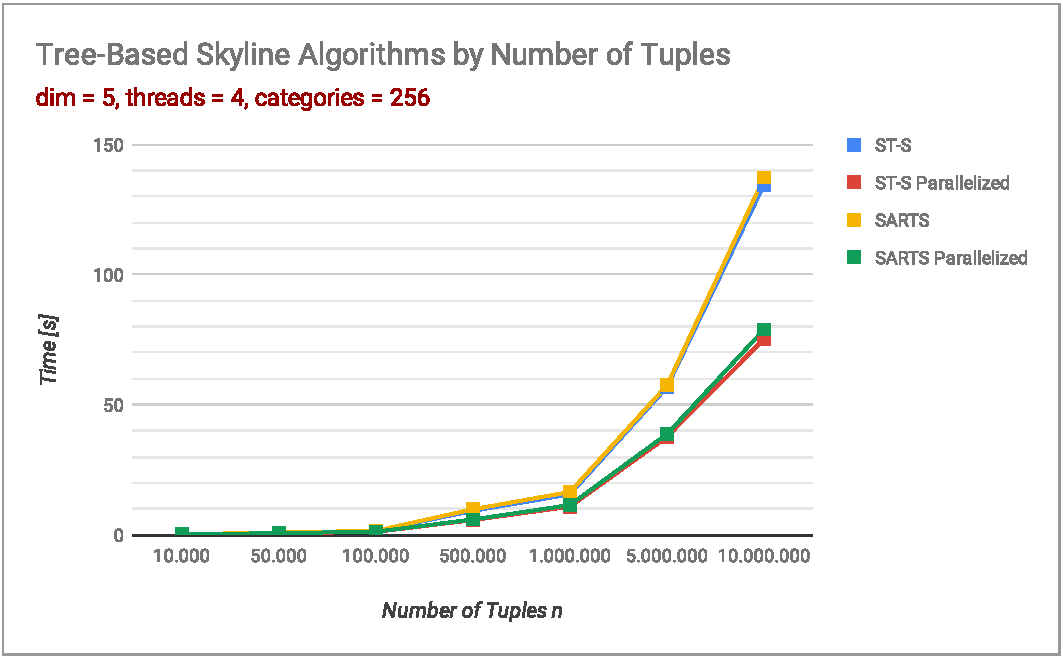
\includegraphics[width=1\linewidth]{figures/progressive-n-2}
	\caption{Running Time of Tree-Based Progressive Algorithms by Number of Tuples}
	\label{fig:progressive-n-2}
\end{figure}

When looking at the results of scaling with dimensionality, a somewhat different picture emerges (Fig.~\ref{fig:progressive-dim}). In this test, Naive-Nested-Loops significantly outperforms both parallelized and sequential versions of ST-S and SARTS. The reason for this is that radix-based tree structures --- which N-Tree and ART both are --- generally scale badly with longer keys. This is the trade-off they have to take for very efficient scaling with the number of elements inserted. The longer the keys of the dataset are, the higher the tree gets, and the longer it takes to traverse the tree from top to bottom. In the application area of skyline computation, the length of a key corresponds to the dimensionality of a tuple. Hence, the more dimensions the tuples of a dataset have, the less efficient tree-based dominance checks become. This is exactly what can be seen in Fig.~\ref{fig:progressive-dim}. 
It also explains why parallelized versions of the algorithms perform worse than the sequential ones. The parallelization of ST-S and SARTS is based on multiple sub-trees used to compute subset skylines before merging them into one final skyline. Thus, the sub-trees also underlie the ``curse of dimensionality''. 

% Progressive Algorithms by dim
\begin{figure}[h]
	\centering
	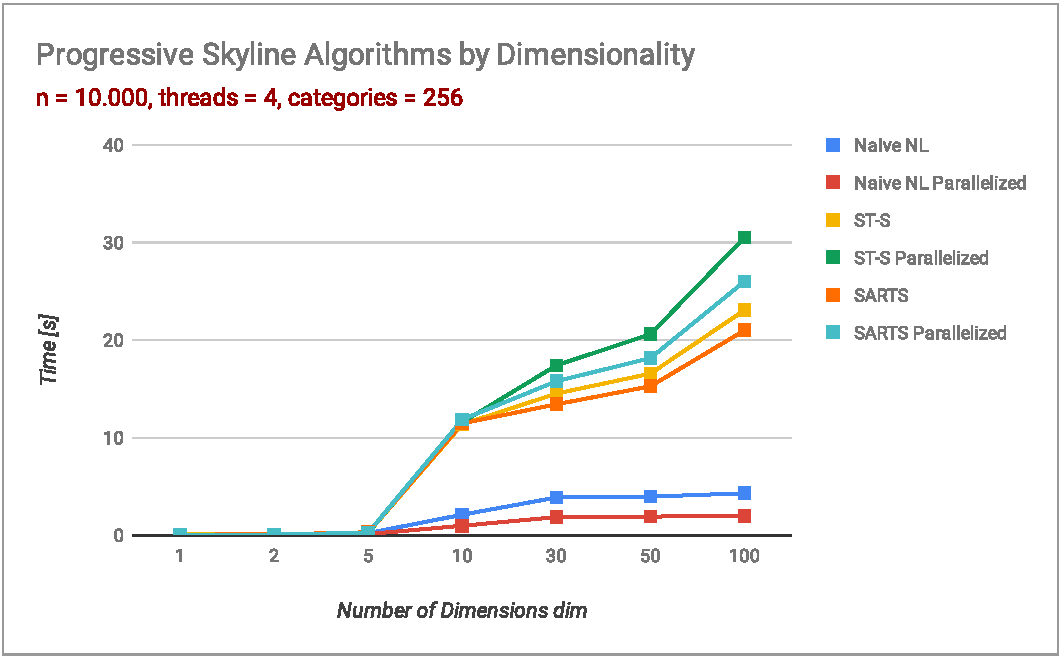
\includegraphics[width=1\linewidth]{figures/progressive-dim}
	\caption{Running Time of Progressive Algorithms by Dimensionality}
	\label{fig:progressive-dim}
\end{figure}

The comparison of progressive algorithms depending on the number of threads available shows that ST-S and SARTS outperform Naive-Nested-Loops for both parallelized and non-parallelized versions. As expected, the time consumption of the parallelized algorithms gets less with a rising number of threads. This means that the parallelization approaches taken in chapter \ref{chapter:Parallelization} produce the desirable performance improvements. While on 1 and 2 threads ST-S and SARTS are a bit faster in their sequential version, on 3 cores and more the parallelized versions show better performance. For the Naive-Nested-Loops algorithm this already happens from 2 threads and up. 
The slightly worse performance of tree-based algorithms on 1 and 2 threads is likely due to the additional overhead required to partition the original dataset, to create a sub-tree for each of the threads, as well as to set up the threads themselves. The performance improvements are expected to become more noticeable if the algorithms run on more than 4 threads, like for instance 8 or 16. 

% Progressive Algorithms by threads
\begin{figure}[h]
	\centering
	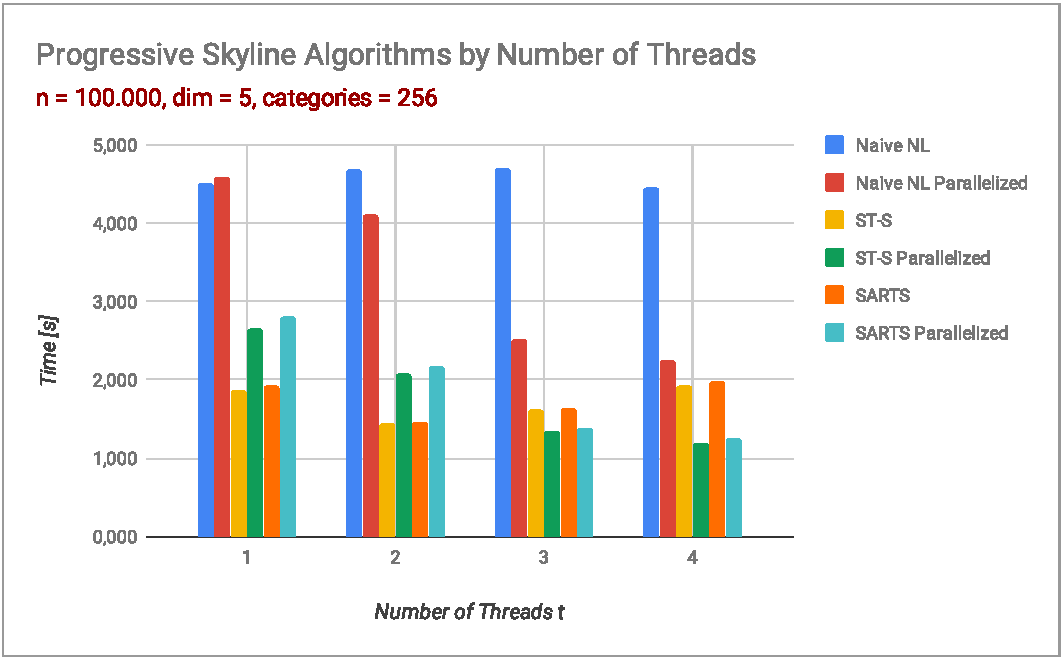
\includegraphics[width=1\linewidth]{figures/progressive-threads}
	\caption{Running Time of Progressive Algorithms by Number of Threads}
	\label{fig:progressive-threads}
\end{figure}

\subsection{Memory Usage}
Within the last two tests, the main memory usage of the ART tree was compared to that of the N-Tree. 
Fig.~\ref{fig:memory-usage-n} shows that the ART tree has significantly lower space consumption than the N-Tree for every $n$ in test. While for $n$ = 10 ART uses about 22-times less memory than N-Tree, even for large $n$, such as $10^{6}$, it still uses appx. 20-times less space than N-Tree. The measured numbers can be found in Appendix \ref{appendix-performance} to this work. 

% memory usage by n
\begin{figure}[h]
	\centering
	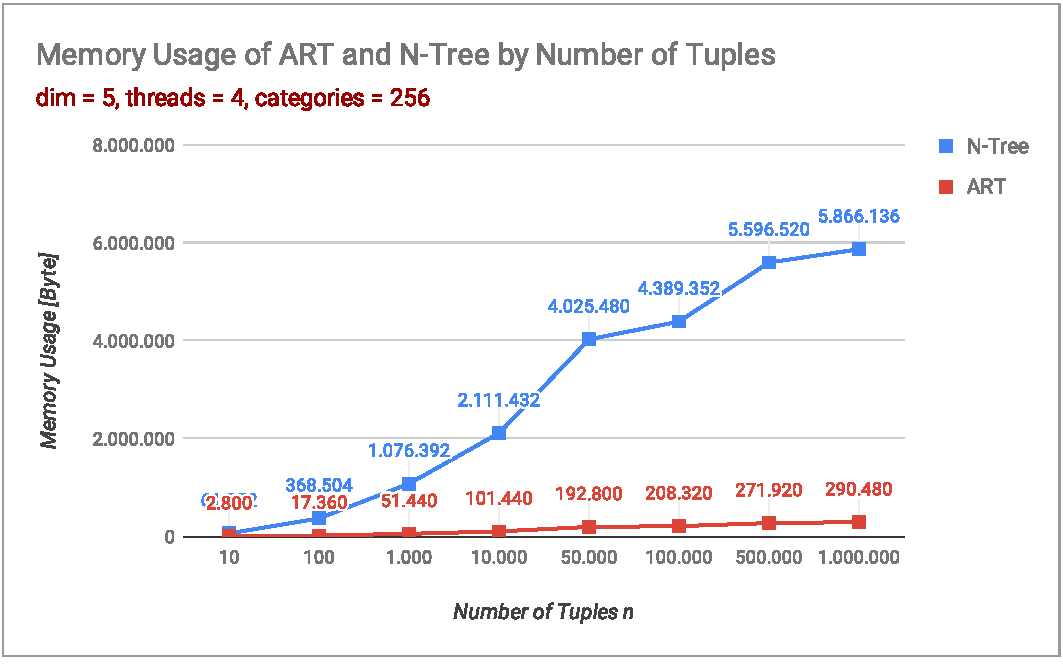
\includegraphics[width=1\linewidth]{figures/memory-usage-n}
	\caption{Memory Usage of ART and N-Tree by Number of Tuples}
	\label{fig:memory-usage-n}
\end{figure}

A similar picture can be seen when looking at memory consumption scaling with dimensionality in Fig.~\ref{fig:memory-usage-dim}. While for low numbers of $dim$, the ART tree already performs better than the N-Tree, it generally scales much more efficiently with high dimensionality. At the point of $dim$ = 50 the ART uses only around $\frac{1}{38}$ of the memory that N-Tree does. Thus, it can be concluded that the SARTS algorithm is significantly more memory-efficient than ST-S due to the usage of ART. 

% memory usage by dim
\begin{figure}[h]
	\centering
	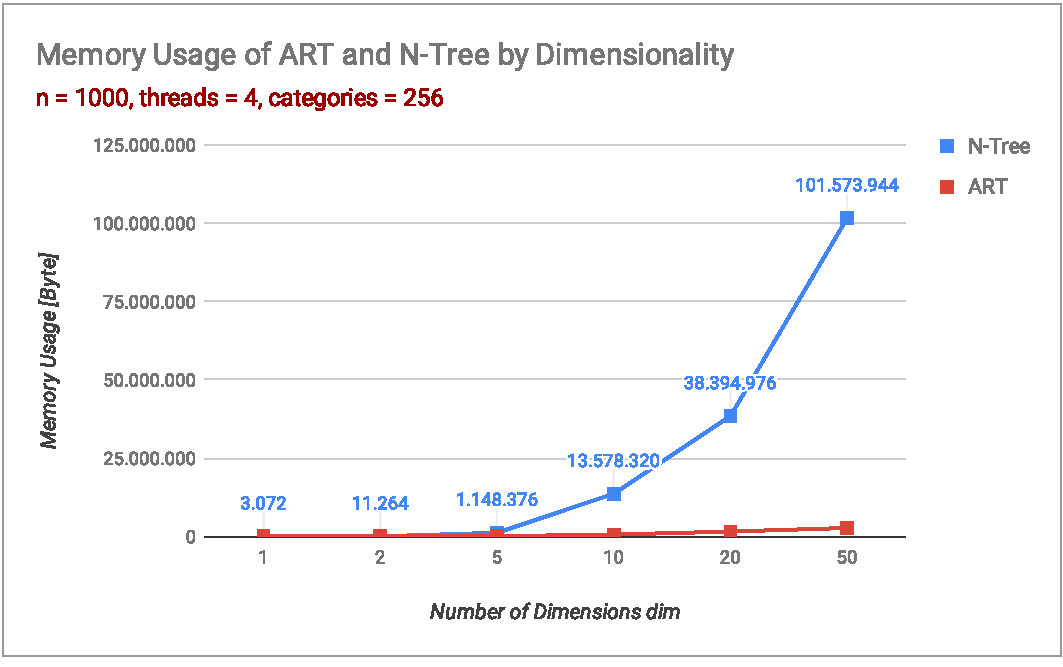
\includegraphics[width=1\linewidth]{figures/memory-usage-dim}
	\caption{Memory Usage of ART and N-Tree by Dimensionality}
	\label{fig:memory-usage-dim}
\end{figure}



